\documentclass[11pt,a4paper,sans]{moderncv}

%% ModernCV themes
\moderncvstyle{casual}
\moderncvcolor{black}
\renewcommand{\familydefault}{\sfdefault}
\nopagenumbers{}
\newcommand{\tab}{\hspace{0.3cm}}

\definecolor{blue}{rgb}{0.0,0.5,1.0}
\definecolor{orange}{rgb}{1.0,0.55,0.0}
\definecolor{green}{rgb}{0,0.8,0.25}
\definecolor{DarkOrchid}{rgb}{0.6, 0.2, 0.8}

%% Character encoding
\usepackage[utf8]{inputenc}

%% Adjust the page margins
\usepackage[inner=2.4cm,outer=2.4cm,top=2cm,bottom=3.0cm,scale=0.75]{geometry}
\usepackage{lscape}
\usepackage{pgfgantt}
\usepackage{xcolor}
\usepackage{natbib}
\usepackage[dutch]{babel}
%\usepackage[]{hyperref}

%% Personal data
\firstname{Cha\"im}
\familyname{De Mulder}
\title{}
\address{Klyvaregr\"and 2/1208}{211 75 Malmö -- Zweden}
\mobile{+32 479 74 55 02}
\email{chaimdemulder@e.email}
%\homepage{www.johndoe.com}
\extrainfo{Geboren 27/3/1991 te Gent}
\photo[76pt][0.8pt]{../images/chaim.jpg}
%\quote{Some quote (optional)}

%%------------------------------------------------------------------------------
%% Content
%%------------------------------------------------------------------------------
\begin{document}
\makecvtitle
\flushright
\vspace{-1.8cm}
\href{https://www.linkedin.com/in/chaimdemulder/}{
\includegraphics[width=0.047\textwidth]{../images/LinkedIn.png}}
%%%%%%%%%%%%%%%%%%%%%%%%%%%%%%%%%%%%%%%%%%%%%%%%%%%%%%%%%%%%%%%%%%%%%%%%%%%%%%
\colorbox{white}{
	\begin{minipage}{\textwidth}
		\section{Ik ben op zoek naar...}
		\cvitem{}{... de mogelijkheid om mijn analytische mindset, mijn technische achtergrond, maar vooral mijn engagement voor een economie ten dienste van mens en de natuurlijke omgeving in te zetten om bij te dragen aan de wereld van morgen.}
	\end{minipage}
}
\vfill
\colorbox{orange!10}{
	\begin{minipage}{\textwidth}
		\section{\textcolor{orange}{\textbf{Werkervaring}}}
		\cventry{\footnotesize Nov. 2019 -- nu}{Energy Management System Engineer}{\footnotesize DuCoop (50\%) \& OpenMotics/Renson Ventilation (50\%), remote tewerkstelling vanuit Zweden}{}{}{}
		\cvitem{}{\small Ontwikkeling en implementatie van een energiemanagementsysteem voor energieco\"operatie \href{https://ducoop.be}{\underline{DuCoop}} in \href{https://denieuwedokken.be}{\underline{De Nieuwe Dokken (Gent)} in het kader van verschillende Europese Horizon 2020 onderzoeksprojecten.}}
		%opvolging van inspraak cooperanten in technologie-ontwikkeling
		\vspace{0.2cm}
		
		\cventry{\footnotesize Okt. 2015 -- Mei 2019}{Doctoraatsstudent}{\footnotesize Universiteit Gent, Faculteit Bioingenieurswetenschappen, Department Data-analyse and Wiskundinge Modellering, BIOMATH (Model-gebaseerde analyse en optimalisatie van bioprocessen)}{}{}{}
		\cvitem{}{\small Titel \href{https://biblio.ugent.be/publication/8621716}{\underline{doctoraat}}: Optimalisatie van databehandeling en hydrodynamische modelstructuur van de rioolwaterzuiveringsinstallatie te Eindhoven.} 
			%\href{https://github.com/UGentBiomath/wwdata}{\underline{wwdata}})}
		\vspace{0.2cm}
		
		\cventry{\footnotesize Okt. 2014 -- Okt. 2015}{Onderzoeksassistent}{\footnotesize Universiteit Gent, Faculteit Bioingenieurswetenschappen, Department Data-analyse and Wiskundinge Modellering, BIOMATH}{}{}{}
		\vspace{0.2cm}
		
		\cventry{\footnotesize Jul. -- Aug. 2013}{Stage master thesis}{\footnotesize DC Water, Research and Development Department}{\footnotesize Washington DC, USA}{}{}
		\vspace{0.2cm}
		
		\cventry{\footnotesize Jul. - Aug. 2012}{IAESTE stage}{\footnotesize Aalto University, Department of Biotechnology and Chemical Technology}{\footnotesize Espoo, Finland}{}{}
		
	\end{minipage}
}
\vfill
%%%%%%%%%%%%%%%%%%%%%%%%%%%%%%%%%%%%%%%%%%%%%%%%%%%%%%%%%%%%%%%%%%%%%%%%%%%%%%
\colorbox{DarkOrchid!10}{
	\begin{minipage}{\textwidth}
		\section{\textcolor{DarkOrchid}{Vaardigheden}}
		\cvitem{Soft skills}{$\bullet$ Analytisch, effici\"ent en gestructureerd}
		\cvitem{}{$\bullet$ Team-geori\"enteerd}
		%Engagerad milj\"o-ingenj\"or} med stort /  och breda intressen;\newline brinner mest f\"or \textbf{milj\"o- och klimatfr\aa gor.
		%\vspace{-.55cm}
		%\cvlistitem{Social och \textbf{storsint}}
		%\cvlistitem{Team-worker}
		%\cvitem{}{$\bullet$ }% och entydig kommunikation} i b\aa de ensamt och samarbete}%, och d\"arf\"or ocks\aa\ van vid bra \textbf{time management}. Stor fokus p\aa\ \textbf{}
		%\cvitem{}{$\bullet$ Grundl\"aggande kunskaper inom \textbf{project management}.}
		%\cvitem{}{$\bullet$ Social och storsint}
		\vspace{0.2cm}
		
		\cvitem{Software/IT}{$\bullet$ Geavanceerd: Python (o.a. Django, Pandas), Git, Docker}
		\cvitem{}{$\bullet$ Basis: MS Office, Google Drive, Teams}
		\vspace{0.2cm}
		\cvitem{Talen}{
			\begin{tabular}{ll}
				$\bullet$ Nederlands (moedertaal) & \tab $\bullet$ Engels (vloeiend)\\
				$\bullet$ Zweeds (vloeiend) & \tab $\bullet$ Frans (basiskennis)\\	
		\end{tabular}}
	\end{minipage}
}
\vfill
%%%%%%%%%%%%%%%%%%%%%%%%%%%%%%%%%%%%%%%%%%%%%%%%%%%%%%%%%%%%%%%%%%%%%%%%%%%%%%
\colorbox{blue!10}{
	\begin{minipage}[]{\textwidth}
		\section{\textcolor{blue}{\textbf{Opleiding}}}
		\cventry{\footnotesize 2009--2014}{Master in de Bioingenieurswetenschappen: Milieutechnologie}{Universiteit Gent}{}{}{}
	\end{minipage}
}
\vfill
%%%%%%%%%%%%%%%%%%%%%%%%%%%%%%%%%%%%%%%%%%%%%%%%%%%%%%%%%%%%%%%%%%%%%%%%%%%%%%
\colorbox{green!10}{
	\small
	\begin{minipage}{\textwidth}
		\section{\textcolor{green}{\textbf{Vrijwillig engagement en cursussen}}}
		\cvitem{}{\textbf{Leiderschap, eenduidige communicatie en doelgericht samenwerken} zijn een aantal van de belangrijkste vaardigheden die mijn engagement mij bijgebracht hebben, naast een diepe overtuiging dat \textbf{een sociaal-ecologische transformatie van onze maatschappij} nodig en mogelijk is. Klik op het logo als je meer wil weten over een specifieke organisatie of vereniging.\newline}
		\cvitem{}{\textbf{Vrijwillig engagement\newline}}
		
		\cventry{\centering\raisebox{-0.4\height}{\href{https://demokratiskomstallning.se}{
\includegraphics[width=0.097\textwidth]{../images/logoDemokratiskOmstallning}}}}{\textbf{Demokratisk Omställning}}{Organisatie van events voor het delen van kennis omtrent municipalisme en democratie (2022 -- nu)}{}{}{}
		\vspace{0.2cm}
		
		\cventry{\centering\raisebox{-0.5\height}{\href{http://degrowth.se}{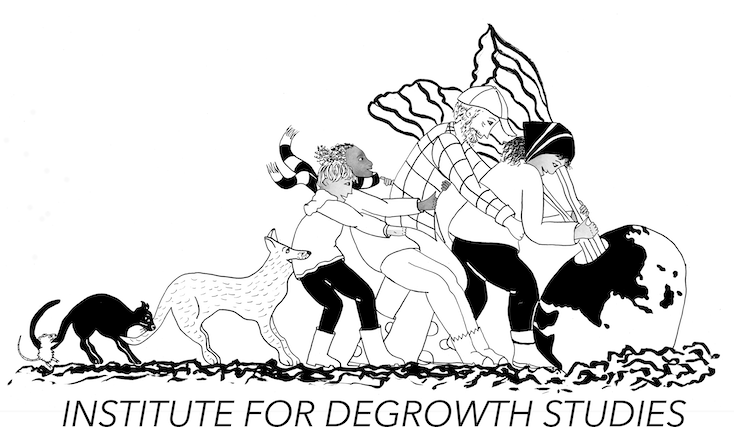
\includegraphics[width=0.097\textwidth]{../images/logoInstituteForDegrowthStudies}}}}{\textbf{The Institute for Degrowth Studies}}{Verspreiden van kennis omtrent degrowth (ontgroei) onder de leden van de vereniging en het brede publiek (2020 -- nu)}{}{}{}
		\vspace{0.2cm}
		
		\cventry{\centering\raisebox{-0.4\height}{\href{http://pushsverige.se}{
\includegraphics[width=0.097\textwidth]{../images/PUSHSverige}}}}{\textbf{PUSH Sverige}}{Zweedse jongerenorganisatie die druk zet op de politiek op Zweeds, Europees en internationaal niveau voor een beter klimaatbeleid (2020 -- 2022)}{}{}{}
		\vspace{0.2cm}
		
		\cventry{\centering\raisebox{-0.4\height}{\href{http://climate-express.be}{
\includegraphics[width=0.057\textwidth]{../images/ClimateExpress}}}}{\textbf{Climate Express}}{Organisatie van kleine en grote klimaatmobilisaties (2018--2019)}{}{}{}
		\vspace{0.2cm}
		
		\cventry{\centering\raisebox{-0.4\height}{\href{https://www.climateresponse.eu}{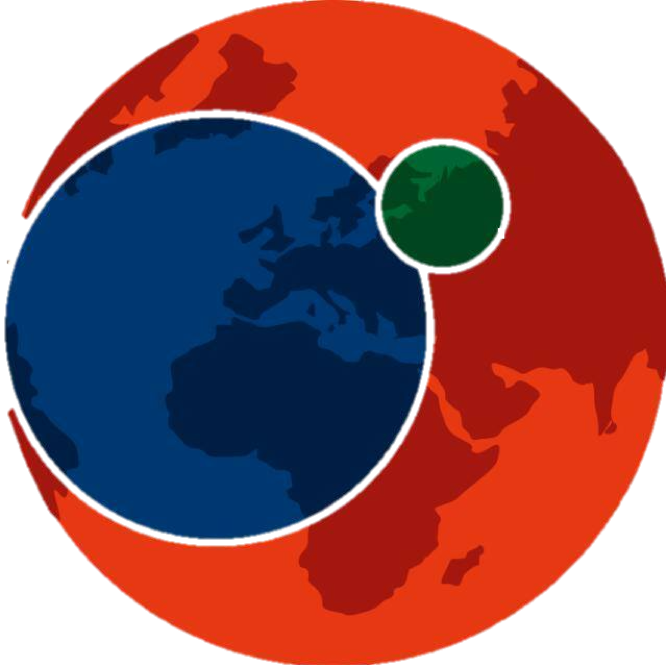
\includegraphics[width=0.055\textwidth]{../images/ClimateResponse.png}}}}{\textbf{Climate Response}}{Voordrachten over de klimaatcrisis: de wetenschappelijke achtergrond en mogelijke oplossingen (2018--2019)}{}{}{}
		\vspace{0.2cm}
		
		\cventry{\centering\raisebox{-0.4\height}{\href{https://www.yaku.be}{
\includegraphics[width=0.06\textwidth]{../images/yaku.png}}}}{\textbf{YAKU}}{Streeft naar het recht op zwemmen in proper water in de stad Gent (2018--2019)}{}{}{}
		\vspace{0.2cm}
		
		\cventry{\centering\raisebox{-0.5\height}{\href{https://iwa-network.org}{
\includegraphics[width=0.06\textwidth]{../images/IWA.png}}}}{\textbf{International Water Association} (IWA)}{Internationaal netwerk voor de watersector (2015--2019)}{}{}{}
		\vspace{0.2cm}
		
		\cventry{\centering\raisebox{-0.7\height}{\href{https://iaeste.org}{
\includegraphics[width=0.06\textwidth]{../images/iaeste_logo}}}}{\textbf{International Association for the Exchange of Students for Technical Experience (IAESTE)}}{Internationale studentenvereninging die stages aanbiedt voor studenten met een technische achtergrond (2013--2018)}{}{}{}
		\vspace{0.5cm}
		
		\cvitem{}{\textbf{Cursussen}}
		\cventry{\centering\raisebox{-0.6\height}{\href{https://www.lunduniversity.lu.se}{
\includegraphics[width=0.073\textwidth]{../images/lunduniversity.png}}}}{Greening the economy -- sustainable cities}{Online cursus aangeboden door Universiteit Lund (26/7/2019 -- 29/8/2019)}{}{}{}
		\vspace{0.2cm}
		\cventry{\centering\raisebox{-0.6\height}{\href{https://ideasforeurope.eu}{
\includegraphics[width=0.097\textwidth]{../images/Coppieters.png}}}}{Climate Action in a Changing Europe}{Cursus aangeboden door de Coppieters Foundation (9/7/2019 -- 11/7/2019)}{}{}{}
		\vspace{0.2cm}
		\cventry{\centering\raisebox{-0.6\height}{\href{https://www.stockholmresilience.org}{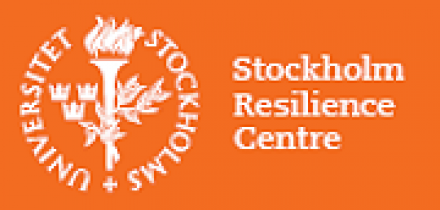
\includegraphics[width=0.097\textwidth]{../images/SRC.png}}}}{Planetary Boundaries and Human Opportunities: the quest for safe and just development on a resilient planet}{MOOC (Massive Open Online Course) aangeboden door het Stockholm Resilience Center (14/9/2015 -- 13/11/2015)}{}{}{}
	\end{minipage}
}
\vfill
%%%%%%%%%%%%%%%%%%%%%%%%%%%%%%%%%%%%%%%%%%%%%%%%%%%%%%%%%%%%%%%%%%%%%%%%%%%%%%
%\section{Overzicht}
%\begin{center}
%	\begin{ganttchart}[
%		hgrid=true,
%		vgrid=true,
%		y unit title=0.8cm,
%		y unit chart=0.5cm,
%		x unit=0.7cm,
%		bar1/.style={bar/.append style={fill=blue}},
%		bar2/.style={bar/.append style={fill=orange}},
%		bar3/.style={bar/.append style={fill=green}}
%		]{1}{18}
%		\ganttset{group height=0.5cm}
%		\gantttitle{\scriptsize{2010}}{1} \gantttitle{\scriptsize{2011}}{1} \gantttitle{2012}{4} \gantttitle{2013}{4} \gantttitle{2014}{4} \gantttitle{2015}{4}\\
%		\textcolor{blue}{\ganttbar[bar1]{Bachelor}{1}{4}}\\
%		\textcolor{blue}{\ganttbar[bar1]{Master}{6}{8}\ganttbar[bar1]{}{10}{12}}\\
%		\textcolor{orange}{\ganttbar[bar2]{IAESTE Stage}{5}{5}}\\
%		\textcolor{orange}{\ganttbar[bar2]{DC Water Stage}{9}{9}}\\
%		\textcolor{orange}{\ganttbar[bar2]{Onderzoeksassistent}{14}{18}}\\
%		\textcolor{green}{\ganttbar[bar3]{IAESTE}{10}{18}}\\
%		\textcolor{green}{\ganttbar[bar3]{Atletiek}{1}{18}}
%	\end{ganttchart}
%\end{center}

%%%%%%%%%%%%%%%%%%%%%%%%%%%%%%%%%%%%%%%%%%%%%%%%%%%%%%%%%%%%%%%%%%%%%%%%%%%%%%
%\section{Personal}
%\cvitem{}{I am a \textbf{motivated and enthusiastic} young man, looking for a \textbf{challenging and diversified} job. During both my working experiences so far, I found that contact with colleagues is something I really appreciate. I am convinced that \textbf{working in a team} with people of different backgrounds can yield better results and more creative engineering solutions.\newline Since I believe I have \textbf{strong values}, I am looking for an employer whose vision I can easily identify with. It goes without saying that I will be even more eager to show a \textbf{committed engagement} working for a company that appeals to me.}

%Obviously, I am ready to show a \textbf{commited engagement} in such a context. }
%\cvitem{Looking for}{Challenging and diversified job, team-work, employer vision and mission I can identify with}

%%%%%%%%%%%%%%%%%%%%%%%%%%%%%%%%%%%%%%%%%%%%%%%%%%%%%%%%%%%%%%%%%%%%%%%%%%%%%%
%\section{Publications}
%\nocite{*}
\nocite{Seuntjens2015}
\nocite{Rehman2015b}
\nocite{Seuntjens2014}
%\biboptions{sort&compress}
\bibliographystyle{bibliodutch} %of bibliodutch, apalike, ieeetr, plainnat...
\bibliography{./CVbiblio}

%%%%%%%%%%%%%%%%%%%%%%%%%%%%%%%%%%%%%%%%%%%%%%%%%%%%%%%%%%%%%%%%%%%%%%%%%%%%%%
%\section{Languages}
%\cvitem{Native}{Dutch}
%\cvitem{Fluent}{English}
%\cvitem{Basic}{French}

%\bibliography{publications}
\end{document}